%
% aufloesung.tex
%
% (c) 2019 Prof Dr Andreas Müller, Hochschule Rapperswil
%
\begin{frame}[fragile]
\frametitle{Funktionenräume}

\begin{definition}
Ein {\em Funktionenraum} $V$ ist ein Vektorraum von Funktionen.
Insbesondere gilt $\forall f,g\in V$ und $\forall \alpha,\beta\in\mathbb C$
\[
\alpha f + \beta g \in V
\]
\end{definition}

\uncover<2->{
\begin{beispiel}
\begin{columns}[T]
\begin{column}{0.34\hsize}
\begin{tikzpicture}[>=latex]
\draw[->,line width=0.7pt] (-0.1,0)--(4.5,0) coordinate[label={$t$}];
\draw[->,line width=0.7pt] (0,-0.1)--(0,2.3) coordinate[label={right:$\varphi$}];

\def\phikurve#1#2#3{
	\fill[color=red!10] ({#1},0)--({#2},0)--({#2},{2*#3})--({#1},{2*#3})
		--cycle;
	\draw[line width=0.7pt] ({#1},0)--({#2},0);
	\draw[color=red,line width=1pt]   (-0.1,0)--({#1},0);
	\draw[color=red,line width=0.1pt] ({#1},0)--({#1},{2*#3});
	\draw[color=red,line width=1pt]   ({#1},{2*#3})--({#2},{2*#3});
	\draw[color=red,line width=0.1pt] ({#2},{2*#3})--({#2},0);
	\draw[color=red,line width=1pt]   ({#2},0)--( 4.3,0);
	\node at ({0.5*(#1+#2)},{#3}) {$T_{#1}\varphi$};
	\node[color=red] at ({0.5*(#1+#2)},{2*#3}) [above] {$a_{0,#1}$};
}

\def\phitrail#1#2#3{
	%\fill[color=red!10] ({#1},0)--({#2},0)--({#2},{2*#3})--({#1},{2*#3})
	%	--cycle;
	%\draw[line width=0.7pt] ({#1},0)--({#2},0);
	%\draw[color=red,line width=1pt]   (-0.1,0)--({#1},0);
	\draw[color=blue,line width=0.1pt] ({#1},0)--({#1},{2*#3});
	\draw[color=blue,line width=1pt]   ({#1},{2*#3})--({#2},{2*#3});
	\draw[color=blue,line width=0.1pt] ({#2},{2*#3})--({#2},0);
	%\draw[color=red,line width=1pt]   ({#2},0)--( 4.3,0);
	\node[color=blue] at ({0.5*(#1+#2)},{2*#3}) [above] {$a_{0,#1}$};
}

\only<2>{
	\phikurve{0}{1}{0.7}
}
\only<3>{
	\phitrail{0}{1}{0.7}
	\phikurve{1}{2}{0.3}
}
\only<4>{
	\phitrail{0}{1}{0.7}
	\phitrail{1}{2}{0.3}
	\phikurve{2}{3}{0.6}
}
\only<5>{
	\phitrail{0}{1}{0.7}
	\phitrail{1}{2}{0.3}
	\phitrail{2}{3}{0.6}
	\phikurve{3}{4}{0.5}
}
\only<6->{
	\phitrail{0}{1}{0.7}
	\phitrail{1}{2}{0.3}
	\phitrail{2}{3}{0.6}
	\phitrail{3}{4}{0.5}
}

\foreach \x in {1,...,4}{
	\draw[line width=0.7pt] ({\x},-0.1)--({\x},0.1);
	\node at ({\x},0) [below] {$\x$};
}
\draw[line width=0.7pt] (-0.1,2)--(0.1,2);
\node at (0,2) [left] {$1$};

\end{tikzpicture}
\end{column}
\begin{column}{0.51\hsize}
\begin{align*}
V_0
&=\left\{
\only<2>{\color{red}} a_{0,0}T_0\varphi \only<2>{\color{black}}
+
\only<3>{\color{red}} a_{0,1}T_1\varphi \only<3>{\color{black}}
+
\only<4>{\color{red}} a_{0,2}T_2\varphi \only<4>{\color{black}}
+\dots
\,
|
\,
a_{0,k}\in\mathbb C
\right\}
\\
&\uncover<5->{=
\left\{
\left.
\sum_{k\in\mathbb Z}a_{0,k}T_k\varphi
\,
\right|
\,
a_{0,k}\in\mathbb C\;\forall k\in\mathbb Z
\right\}
}
\\
&\uncover<6->{=
\left\langle
T_k\varphi\,|\;k\in\mathbb Z
\right\rangle
}
\end{align*}
\end{column}
\end{columns}
\bigskip

\uncover<7->{
Jedes mit Rate $1$ abgetastete Signal ist in $V_0$.
}
\end{beispiel}
}

\end{frame}

\let\phikurve\undefined
\let\phitrail\undefined

%
% Höhere Auflösung
%
\begin{frame}[fragile]
\frametitle{Skala $\frac12$\uncover<27->{ und kleiner: $2^{-j}$}}
\begin{center}
\begin{tikzpicture}[>=latex]

\def\faktor{19.1}

\draw[->,line width=0.7pt] (0,-0.1)--(0,2.5) coordinate[label={right:$f$}];

\def\phikurve#1#2#3{
	\fill[color=red!10] ({0.5*#1},0)--({0.5*#2},0)--({0.5*#2},{2*#3})
		--({0.5*#1},{2*#3})--cycle;
	\draw[line width=0.7pt] ({0.5*#1},0)--({0.5*#2},0);
	\draw[color=red,line width=1pt]   (-0.1,0)--({0.5*#1},0);
	\draw[color=red,line width=0.1pt] ({0.5*#1},0)--({0.5*#1},{2*#3});
	\draw[color=red,line width=1pt]   ({0.5*#1},{2*#3})--({0.5*#2},{2*#3});
	\draw[color=red,line width=0.1pt] ({0.5*#2},{2*#3})--({0.5*#2},0);
	\draw[color=red,line width=1pt]   ({0.5*#2},0)--(12.3,0);
	\node at ({0.25*(#1+#2)},0) [below] {$T_{#1}\varphi$};
	\node[color=red] at ({0.25*(#1+#2)},{2*#3}) [above] {$a_{0,#1}$};
}

\def\phitrail#1#2#3{
	\draw[color=blue,line width=0.1pt] ({0.5*#1},0)--({0.5*#1},{2*#3});
	\draw[color=blue,line width=1pt]   ({0.5*#1},{2*#3})--({0.5*#2},{2*#3});
	\draw[color=blue,line width=0.1pt] ({0.5*#2},{2*#3})--({0.5*#2},0);
	%\node[color=blue] at ({0.25*(#1+#2)},{2*#3}) [above] {$a_{0,#1}$};
}

\only<2>{
	\pgfmathparse{abs(sin(\faktor*(0.25)))}
	\xdef\yvalue{\pgfmathresult}
	\phikurve{0}{1}{\yvalue}
}

\foreach \x in {3,...,25}{
	\only<\x>{
		\pgfmathparse{\x-2}
		\xdef\xlimit{\pgfmathresult}
		\foreach \y in {1,...,\xlimit}{
			\pgfmathparse{\y-1}
			\xdef\xlinks{\pgfmathresult}
			\pgfmathparse{\y}
			\xdef\xrechts{\pgfmathresult}
			\pgfmathparse{abs(sin(\faktor*(\xlinks+0.5)))}
			\xdef\yvalue{\pgfmathresult}
			\phitrail{\xlinks}{\xrechts}{\yvalue}
		}
		\pgfmathparse{\x-2}
		\xdef\xlinks{\pgfmathresult}
		\pgfmathparse{\x-1}
		\xdef\xrechts{\pgfmathresult}
		\pgfmathparse{abs(sin(\faktor*(\xlinks+0.5)))}
		\xdef\yvalue{\pgfmathresult}
		\phikurve{\xlinks}{\xrechts}{\yvalue}
	}
}

\only<26-27>{
	\foreach \y in {1,...,24}{
		\pgfmathparse{\y-1}
		\xdef\xlinks{\pgfmathresult}
		\pgfmathparse{\y}
		\xdef\xrechts{\pgfmathresult}
		\pgfmathparse{abs(sin(\faktor*(\xlinks+0.5)))}
		\xdef\yvalue{\pgfmathresult}
		\phitrail{\xlinks}{\xrechts}{\yvalue}
	}
}

\only<28>{
	\foreach \x in {0.125,0.375,...,12}{
		\draw[color=blue,line width=0.1pt]
			({\x-0.125},0)
			--({\x-0.125},{2*abs(sin(\faktor*(2*\x)))});
		\draw[color=blue,line width=1pt]
			({\x-0.125},{2*abs(sin(\faktor*(2*\x)))})
			--({\x+0.125},{2*abs(sin(\faktor*(2*\x)))});
		\draw[color=blue,line width=0.1pt]
			({\x+0.125},{2*abs(sin(\faktor*(2*\x)))})
			--({\x+0.125},0);
	}
}

\only<29>{
	\foreach \x in {0.0625,0.1875,...,12}{
		\draw[color=blue,line width=0.1pt]
			({\x-0.0625},0)
			--({\x-0.0625},{2*abs(sin(\faktor*(2*\x)))});
		\draw[color=blue,line width=1pt]
			({\x-0.0625},{2*abs(sin(\faktor*(2*\x)))})
			--({\x+0.0625},{2*abs(sin(\faktor*(2*\x)))});
		\draw[color=blue,line width=0.1pt]
			({\x+0.0625},{2*abs(sin(\faktor*(2*\x)))})
			--({\x+0.0625},0);
	}
}
\only<30>{
	\fill[color=blue!10]
		plot[domain=0:12,samples=1000]
			({\x},{2*abs(sin(\faktor*(2*\x)))})--(12,0)--cycle;
	\draw[line width=1pt,color=blue]
		plot[domain=0:12,samples=1000]
			({\x},{2*abs(sin(\faktor*(2*\x)))});
}

\draw[->,line width=0.7pt] (-0.1,0)--(12.5,0) coordinate[label={$t$}];

\foreach \x in {1,...,12}{
	\draw[line width=0.7pt] ({\x},-0.1)--({\x},0.1);
}
\draw[line width=0.7pt] (-0.1,2)--(0.1,2);

\end{tikzpicture}
\end{center}

\begin{align*}
V_1
&=
\left\langle\left. T_kD_{\frac12}\;\right|\; k\in\mathbb Z \right\rangle
\\
&\uncover<27->{\;\;\vdots}
\\
\uncover<27->{V_{\only<27>{1}\only<28>{2}\only<29>{3}\only<30->{j}}}
&\uncover<27->{=
\left\langle\left. T_kD_{2^{\only<27>{-1}\only<28>{-2}\only<29>{-3}\only<30->{-j}}}
\;\right|\; k\in\mathbb Z \right\rangle}
\end{align*}

\end{frame}

